\chapter{Inverse Synthesis Experiment}
\label{chapter:inverse_synth_experiment}

This chapter presents an inverse synthesis experiment that was conducted to compare some of the recent approaches that have been used in previous work. The methodology used for this experiment was modelled after Yee-King et al.'s study on deep learning for automatic synthesizer programming \cite{yee2018automatic}, but with a simplified synthesizer configuration and a unique set of estimators. In total ten different methods for inverse synthesis were compared, including eight deep learning models based on previous work \cite{barkan2019inversynth, yee2018automatic} and two versions of a genetic algorithm \cite{horner1993machine, tatar2016automatic}. A VST software emulation of the Yamaha DX7 FM synthesizer called \textit{Dexed} was used with a restricted subset of the parameters. While Dexed has been used in previous work for inverse synthesis \cite{yee2018automatic, luke2019stochastic, le2021improving, masudo2021quality}, each work has used a unique subset of parameters and sounds for their experiments. Depending on the parameters that are selected, the difficulty of the problem varies considerably. In this experiment we propose a minimal subset of nine parameters to reduce the complexity of the problem and to provide a benchmark for evaluation.

The following section describes in more detail the methods used for this experiment including the precise configuration of the synthesizer, the dataset used for training, and the various techniques compared. Section \ref{sec:inverse-synth-eval} describes the methods used for evaluation and the results of this evaluation. Section \ref{sec:inverse-synth-discuss} presents a discussion of the results and some of the challenges associated with the inverse synthesis problem. In alignment with Vandewalle et al.'s criteria for reproducible research, implementation details, code, and datasets are all available on the \mintinline{python}{spiegelib} online documentation.\footnote{\url{https://spiegelib.github.io/spiegelib/examples/fm_sound_match.html}}

\section{Methods}

\subsection{Synthesizer}
The first step in the experiment was defining the synthesizer setup. The $Dexed$ VST instrument was selected for this experiment for a number of reasons: 1) it is an FM synthesizer that is modelled closely after the Yamaha DX7 synthesizer which is both widely used as well as notoriously difficult to program, 2) Dexed is open-source and free to use which makes it easy for the results to be reproduced, and 3) it has been used in a number of previous works on inverse synthesis \cite{yee2018automatic, luke2019stochastic, le2021improving, masudo2021quality}. An image of the $Dexed$ interface is shown in figure \ref{fig:dexed}. Dexed has 155 automatable parameters that are accessible for control from a DAW, which represent the parameters that are available for programming via inverse synthesis. A subset of nine of these parameters were used in this experiment to turn $Dexed$ into a simple two-operator FM synthesizer. In this configuration the second operator modulates the frequency of the first operator. A block diagram showing the resulting synth configuration is shown in figure \ref{fig:two_op_fm_block}. The subset of nine parameters control the amplitude envelope and tuning of the modulating oscillator; this simple synthesizer can produce a wide range of timbres that evolve in various ways over time based on the amplitude envelope of the modulating oscillator. An overview of these nine parameters is given in table \ref{tbl:dexed-params}.

\begin{figure}[ht]
    \centering
    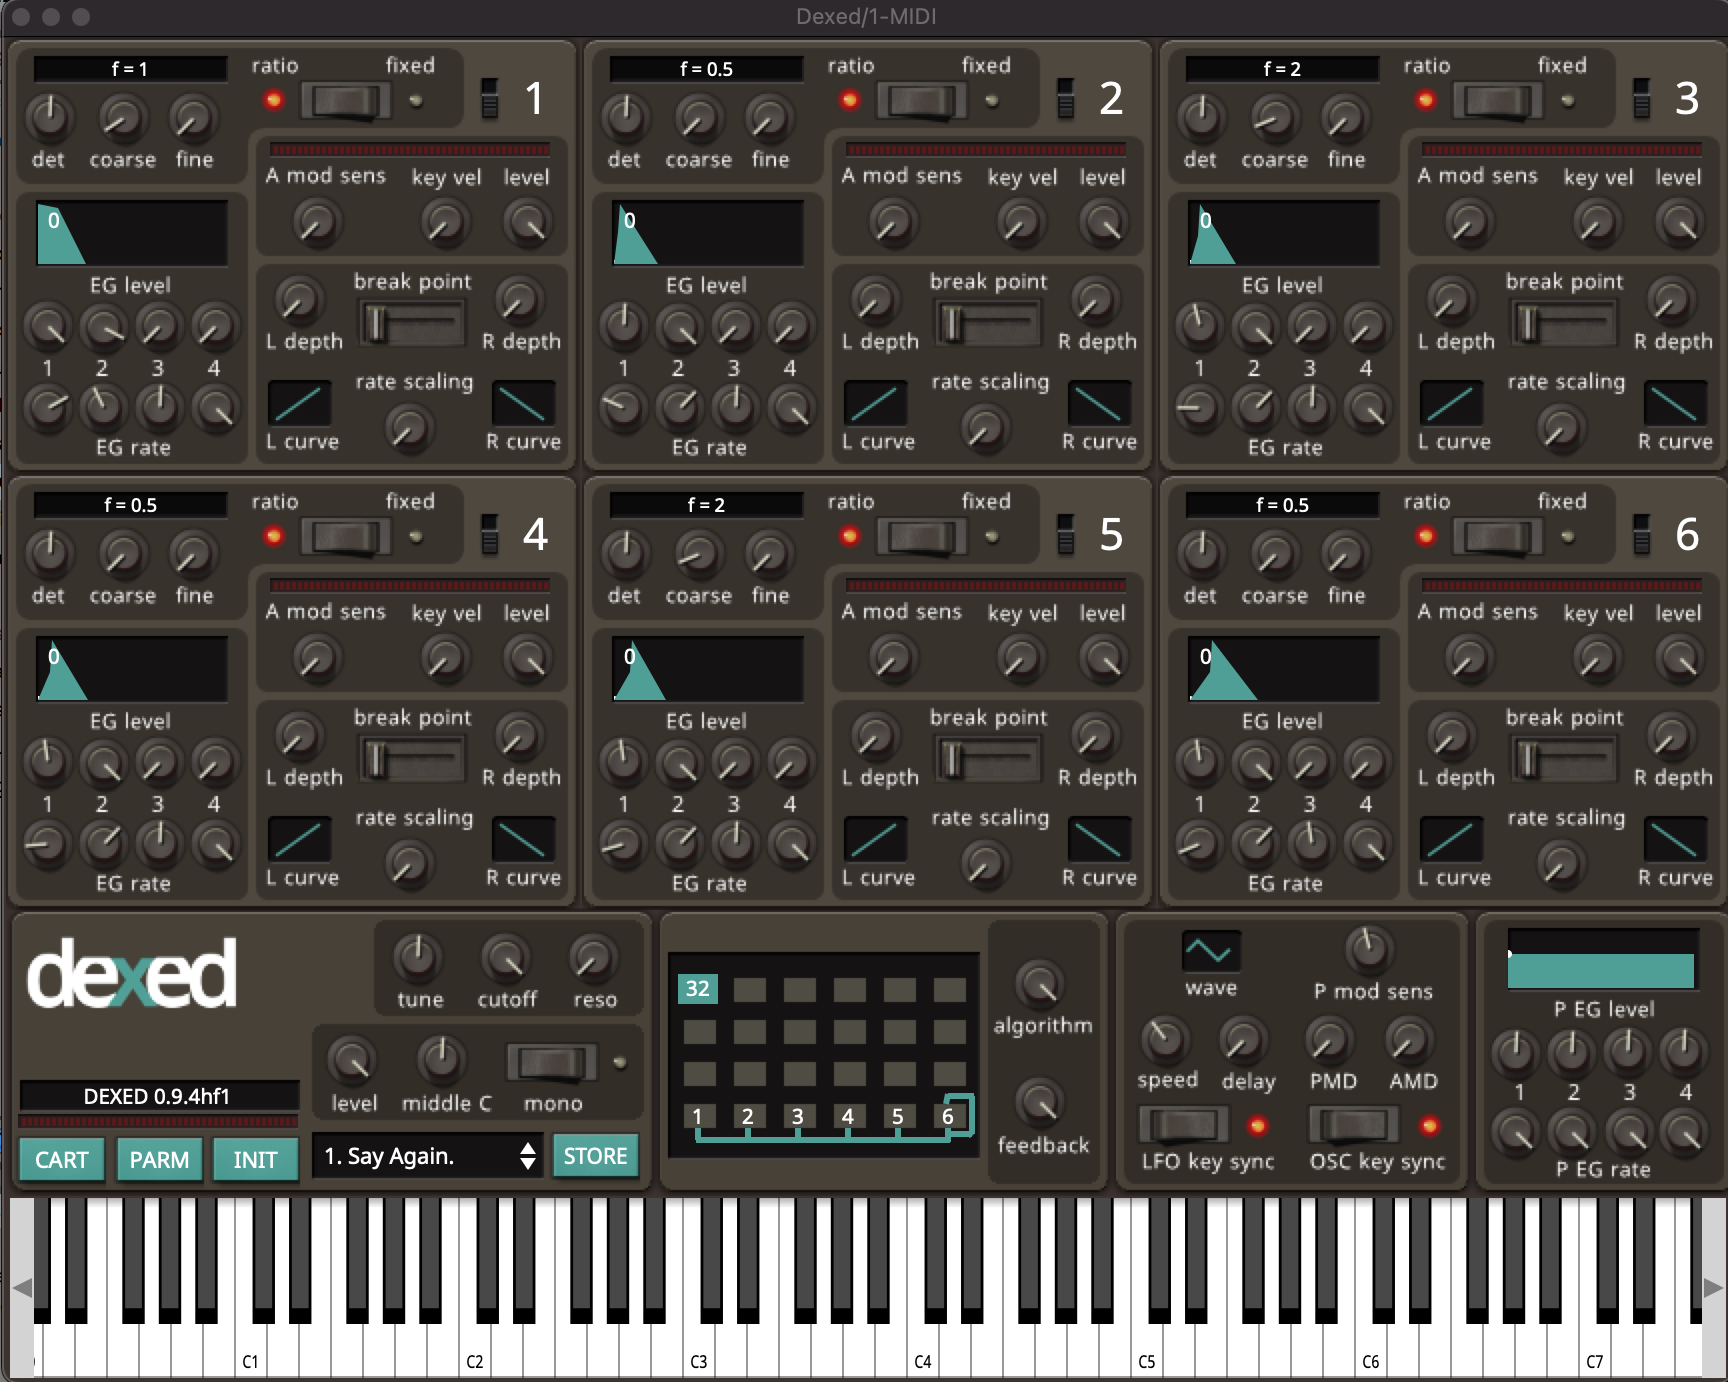
\includegraphics[width=0.6\textwidth]{figures/spiegelib/dexed.png}
    \caption{The Dexed synthesizer interface. Dexed is an open-source emulation of the Yamaha DX7 FM synthesizer and it was used in the experiments in this chapter/}
    \label{fig:dexed}
\end{figure}

\begin{figure}[ht]
    \centering
    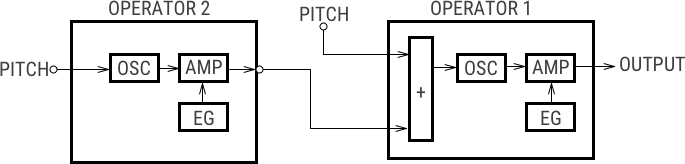
\includegraphics[width=0.9\textwidth]{figures/spiegelib/two_op_fm_block.png}
    \caption{Block diagram of a two operator FM synthesizer. Dexed has six independent operators that can be configured in various ways, however for the experiments conducted here only the first two operators were used and were setup in this configuration.}
    \label{fig:two_op_fm_block}
\end{figure}

\begin{table}[ht]
\centering
\caption{Synthesis parameters used in experiment}
\label{tbl:dexed-params}
%\def\arraystretch{1.5}%  1 is the default, change whatever you need
\begin{tabular}{l|l}
\toprule
Parameter     & Description                                                                                  \\
\midrule
OP2 EG RATE 2 & \multirow{3}{*}{\parbox{0.70\linewidth}{Controls the duration of stages 2-4 of the envelope generator applied the the amplitude of operator 2}} \\
OP2 EG RATE 3 \\
OP2 EG RATE 4 \\
\midrule
OP2 EG LEVEL 2 & \multirow{3}{*}{\parbox{0.6\linewidth}{Controls level of the envelope generator at stages 2-4, which is applied the amplitude of operator 2}} \\
OP2 EG LEVEL 3 \\
OP2 EG LEVEL 4 \\
\midrule
OP2 F COARSE & \multirow{2}{*}{\parbox{0.6\linewidth}{Frequency of second operator in relation to the fundamental frequency of the MIDI pitch. Coarse tuning is an integer ratio from $\frac{1}{2}$ to 31. Fine tuning allows for smaller non-integer adjustments.}} \\[2.75ex]
OP2 F FINE \\[2.75ex]
\midrule
OP2 OSC DETUNE & \multirow{1}{*}{\parbox{0.6\linewidth}{Detunes the second operator by $\pm$ 7 cents}}\\
\bottomrule                                                                                        
\end{tabular}
\end{table}
\vspace{1cm}

Each operator in $Dexed$ has a complex envelope generator (EG) that is used modulate the amplitude of that operator. The complex envelope generator has five independent stages that are controlled by a set of parameters that are used to adjust the length and amplitude of each stage. For this experiment, only the EG for the second operator had parameters for estimation: $LEVEL 2-4$ and $RATE 2-4$. The $RATE 1$ and $LEVEL 1$ parameters were locked to the minmimum rate and highest level, effectively turning off the initial rise portion of the envelope. Three parameters controlling the pitch and tuning of the second operator were also open for estimation. Although each of the included parameters control the amplitude EG and pitch of the operator in distinct ways, there is redundancy in the parameter spaced, i.e. different parameter settings could lead to the same auditory result. This redundancy represents one of the complexities of synthesizer parameter spaces and challenges in automatic synthesizer programming. This experiment intentionally seeks to explore the affect this redundancy has on each techniques ability to effectively match. All parameters have a normalized range from $[0-1]$ and mapping from this normalized range is handled internally by the Dexed code. The remainder of the available parameters in $Dexed$ are locked at values to create a simple sine wave generator that is being frequency modulated by the second operator. [ADD A TABLE IN APPENDIX FOR ALL THE PARAMETER VALUES]. The \mintinline{python}{SynthVST} class in spiegelib provides methods for overriding and freezing parameters as well as saving and loading parameter settings as JSON files. 

\begin{figure}[ht]
    \centering
    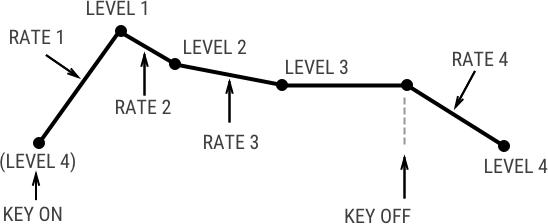
\includegraphics[width=0.75\textwidth]{figures/spiegelib/Yamaha DX7 Envelope.png}
    \caption{Diagram of an envelope generator in the Yamaha DX7 and Dexed. The envelope has five independent stages. During the first three stages the envelope moves linearly from level 4 to level 1, then to level 2, then to level 3. Each of these levels is controllable and the length of time taken to move to each level is also definable. This movement is triggered by a key-on event. Once the envelope has progressed to level 3 it stays at that level until a key-off event is received, at which point the envelope progresses back to level 4.}
    \label{fig:dx7_envelope}
\end{figure}


\subsection{Dataset}
A dataset of synthesized audio paired with the parameters used for generation was required for training the deep learning models used in this experiment. Dataset creation consisted of sampling the parameter space, rendering the audio resulting from the parameters, and then transforming the audio into a suitable audio representation for each model. All audio was rendered by sending a single MIDI note to Dexed with a note value of 48 (C3 - $\approx 130.81$Hz) and length of one second. 60,000 examples were generated by uniformly sampling the nine parameters and rendering audio for one second; audio results were saved as wav files at a sampling rate of 44,100kHz. The parameter values were also saved alongside each example. This dataset was then split into a training and validation set with the training set containing 80\% of the samples. Once the audio dataset was created, audio representations were generated for each example.

\subsubsection{Audio Representations}
All the models received audio input that has been transformed into a more perceptually relevant representation. Two different representations were used. The fully-connected and recurrent models used a 13-band Mel-frequency cepstral coefficient (MFCC) representation, which was the same used by Yee-King \textit{et al.} \cite{yee2018automatic}, and the convolutional neural networks (CNNs) used a log-scaled Mel-spectrogram representation. Barkan \textit{et al.} \cite{barkan2019inversynth} used a STFT representation in their experiments with CNNs, however Mel-spectrograms provide a more perceptually relevant frequency scaling and has been used in recent work in audio representations \cite{cramer:learnmore:icassp:19, hershey2017cnn}.

The MFCCs were computed with 13-bands using a frame size of 2048 and a hop size of 1024, this resulted in 44 frames over the 1-second long input audio. To compute the Mel-spectrograms, a STFT was first computed using a frame-size of 2048 samples and a hop-size of 1024 samples. Each frame of the magnitude spectrogram was then converted to a power spectrum and then projected onto a 128 component Mel-frequency scale. The resulting Mel-spectrogram is then scaled to a log-scale, which is an amplitude scaling more reflective of human auditory perception of loudness. Equation \ref{ref:eq-log-scale} shows the calculation of the log-scaled Mel-spectrogram from a complex valued spectrogram, $\textbf{X}$, where $\textbf{M}$ is a matrix of weights to project each frame in the spectrogram onto 128 Mel-frequency bins.

\begin{align}\label{ref:eq-log-scale}
    \textbf{X}_{logmel} &= 10*log_{10}(|\textbf{X}|^2 \cdot \textbf{M})
\end{align}

MFCC features were standardized to have zero mean and unit variance, and the Mel-spectrograms are treated as grey-scale images and normalized to the range $[0-1]$. An example of the resulting representations computed on a the same audio sample is shown in figure \ref{fig:mfcc-mel-representations}. Both the MFCC and Mel-spectrogram representations show an envelope in the signal starting at the beginning of the sound and lasting until about 0.45 seconds. The Mel-spectrogram gives a much higher resolution perspective of the frequencies present in the signal, whereas the MFCC only captures the overall shape of the spectral envelope and provides a much more compact representation. Pitch information is lost with MFCCs, which was identified by Masuda \textit{et al.} as an issue for synthesizer sound matching applications \cite{masudo2021quality}, however we include them in this experiment since they have lead to success in previous inverse synthesis experiments \cite{yee2018automatic}. Whether the higher-resolution Mel-spectrogram images will allow the models that use them to perform better is another research question.

\begin{figure}[ht]
    \centering
    \begin{subfigure}[b]{0.45\textwidth}
        \centering
        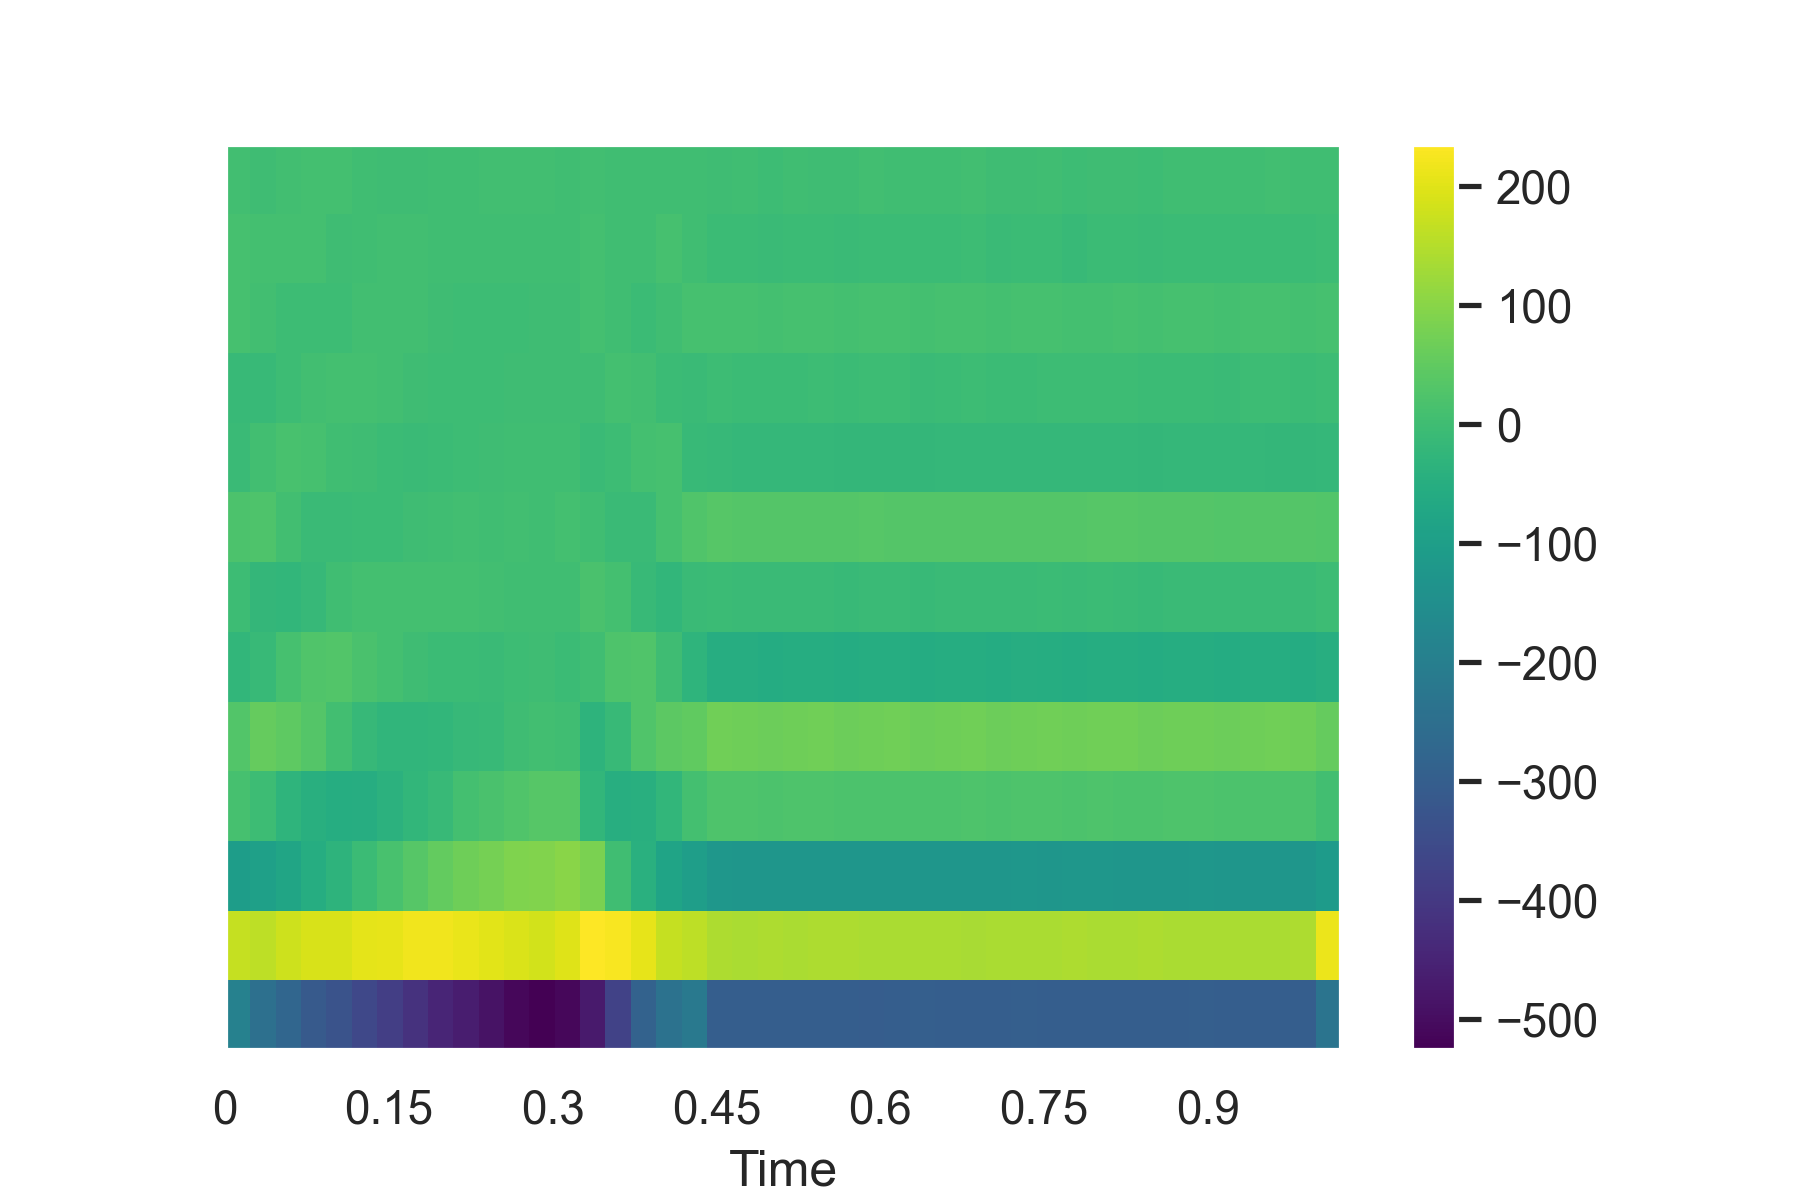
\includegraphics[width=\textwidth]{figures/inverse-synth/features_mfcc_example.png}
        \caption{MFCC}
    \end{subfigure}
    \begin{subfigure}[b]{0.45\textwidth}
        \centering
        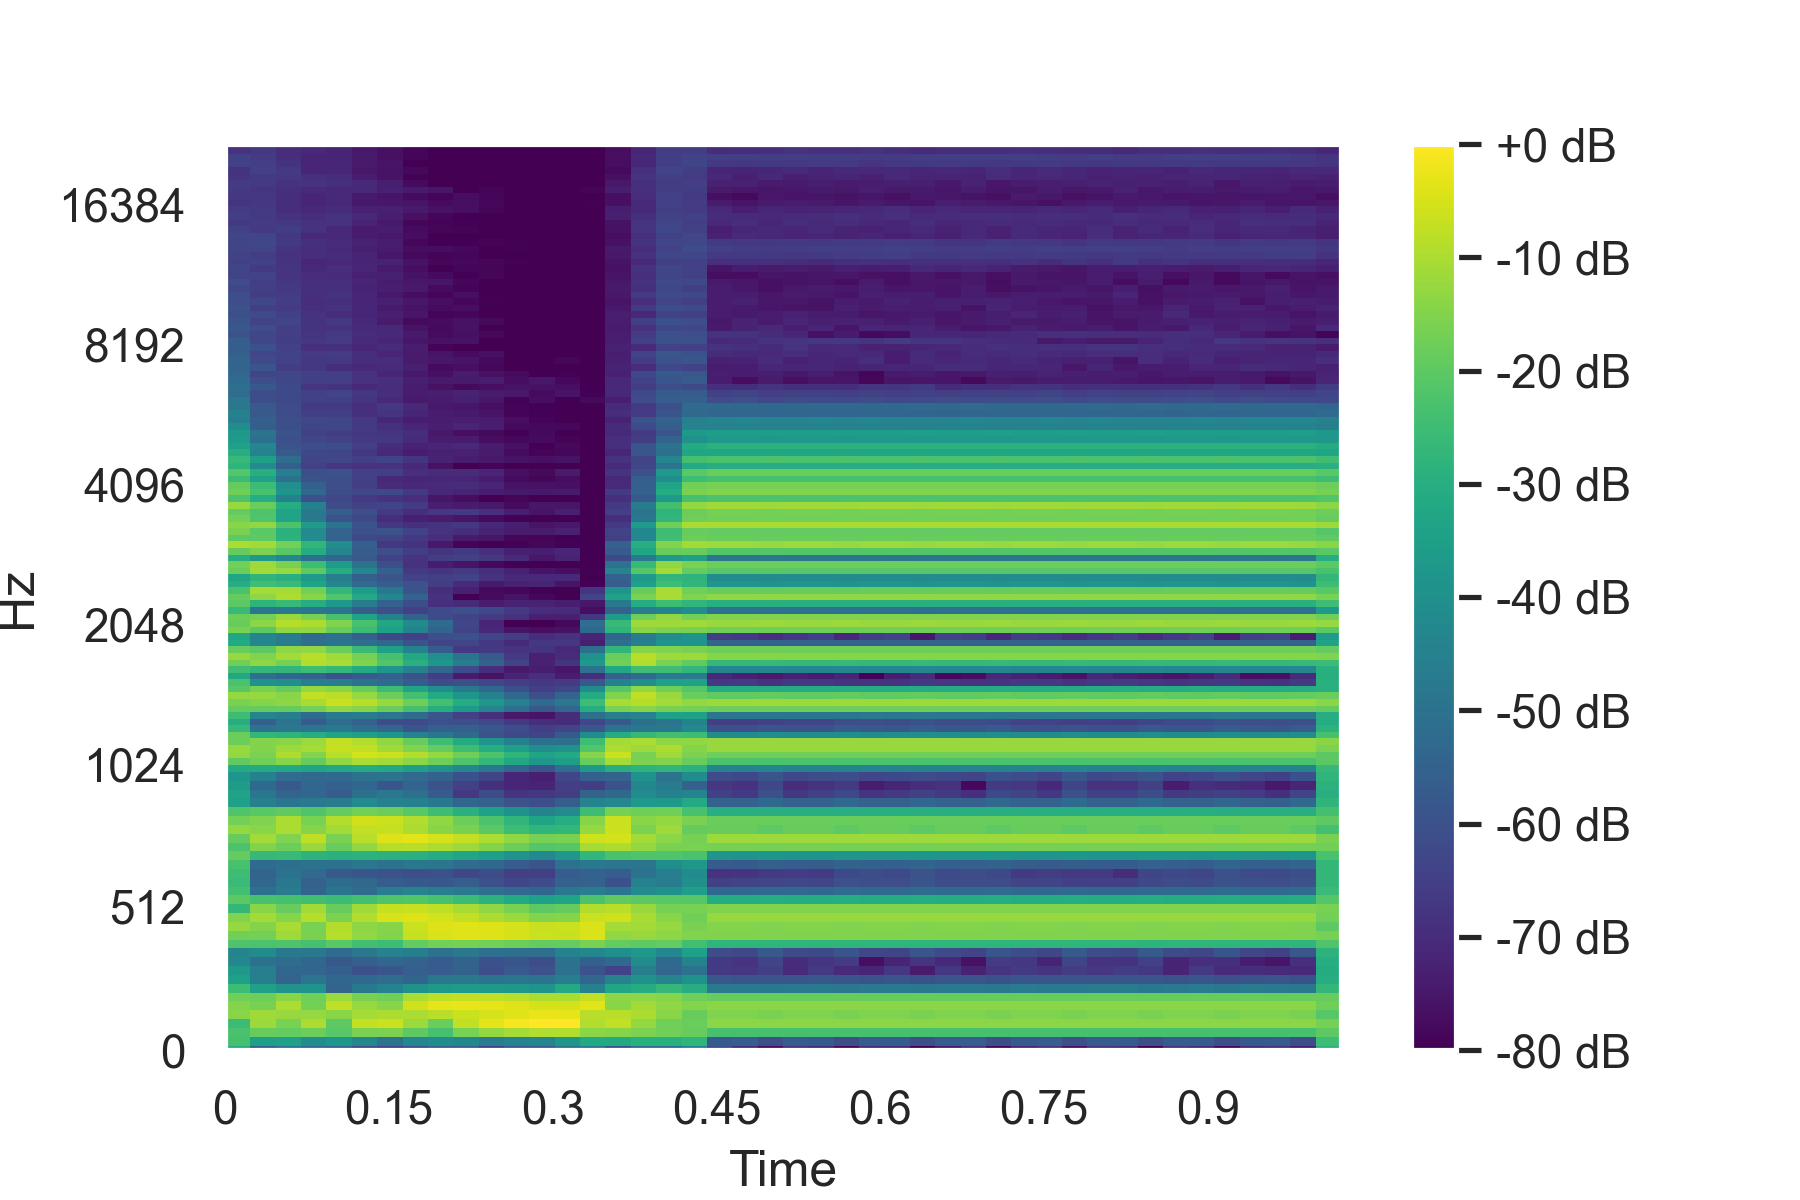
\includegraphics[width=\textwidth]{figures/inverse-synth/features_mel_example.png}
        \caption{Mel-Spectrogram}
    \end{subfigure}
    \caption{Audio representations generated for a single audio example in the dataset. The left figures shows a 13-band MFCC, and the right shows a log-scaled 128-band Mel-Spectrogram.}
    \label{fig:mfcc-mel-representations}
\end{figure}

\subsection{Deep Learning Models}
Eight different models were used in this experiment. Three recurrent neural networks (RNNs) derived from work by Yee-King \textit{et al.} \cite{yee2018automatic}, four convolutional neural networks (CNNs) derived from work by Barkan \textit{et al.} \cite{barkan2019inversynth}, and a baseline multi-layer perceptron (MLP) network, also from Yee-King \textit{et al.} \cite{yee2018automatic}. The RNN models use the time-series of MFCC features as input, the CNN models use the Mel-spectrogram images as input, and the MLP network uses a flattened version of the time-series MFCC features. All models output floating point value estimations for the nine synthesizer parameters. Because these output values can be any 32-bit floating point number (outputs are clipped to a $[0-1]$ range), this means that the models are solving a regression problem. The loss function used during training was the mean squared error (MSE) between the target parameter values $\textbf{y}$ and the predicted parameter values $\hat{\textbf{y}}$. The MSE is calculated as follows, where $N$ is the number of parameters:

\begin{equation}\label{equation:mse}
    \ell(\textbf{y}, \hat{\textbf{y}}) = \frac{\sum_{i \in N}{(y_i - \hat{y_i})^2}}{N}
\end{equation}

Ideally the loss would be calculated on audio produced by Dexed using the estimated parameters, however there are currently no available solutions for rendering audio using VST instruments within a deep learning model and including it in the the training loop. Recent work by Ramírez \textit{et al.} presented a solution for including audio effect plugins within a deep learning networks \cite{ramirez2021differentiable} which could also enable training on VSTis as well, however I leave that for future suggested work. 

Models were trained using an $Adam$ optimizer \cite{kingma2014adam} and hyperparameters for each model were optimized using a  Tree-structured Parzen Estimator (TPE), which has been shown to be an effective method for hyperparameter selection \cite{bergstra2011algorithms}. Early stopping was used during training for all models, this halted training if the validation loss stopped decreasing for a certain number of training epochs. The number of training epochs that early stopping waited before halting training is referred to as $patience$, and was selected based on results from hyperparameter optimization.

The following subsections describe each of the models that were included in this experiment. To find specific details on the implementation of each model see appendix \ref{appendix:spiegelib_models}.

% Maybe not important
%This is a natural way to approach the problem considering the continuous nature of the parameters exposed by a given synthesizer, and this is the approach taken by Yee-King \textit{et al.}. Conversely, Barkan \textit{et al.} framed the inverse synthesis problem as a classification problem by dividing each parameter into 16 classes, which meant that there would be $n*16$ classes, where $n$ is the number of parameters. Quantizing the parameter space into 16 discrete values per parameter 

\subsubsection{Multi-Layer Perceptron}
% Find cites for  the MLP?
Multi-Layer Perceptron (MLP) models, also referred to as a feedforward neural network, were the first and most simple types of neural networks. They contain one or more hidden layers containing neurons that are connected to each neuron in the preceding and proceeding layers. Because of fully connected nature of these layers, they are also referred to as dense layers. An MLP is included in this experiment as a baseline model to benchmark the other models againsts. The architecture for the MLP was derived from Yee-King \textit{et al.} \cite{yee2018automatic} and has three hidden layers containing 50, 40, and 30 neurons respectively. Each neuron utilizes a ReLu activation and the model contains 32k trainable parameters. It was trained using a learning rate of 0.001, a patience of 25 epochs, and a batch-size of 128.

\subsubsection{Recurrent Neural Networks}
% Find cites for these different networks??
Three different Recurrent Neural Networks (RNNs) derived from work by Yee-King \textit{et al.} \cite{yee2018automatic} were used in this experiment:
\begin{itemize}
    \item \textit{LSTM:} The first is an RNN with three LSTM layers, each containing 64 units, followed by a dropout layer with frequency of 0.2 and a fully connected output layer. It contains 86.6k trainable parameters. This is a modified version of the model used by Yee-King, the number of units for each LSTM and the rate of the dropout were both selected through hyperparameter optimization; the main difference is that this model uses only 64 units in each LSTM as opposed to 100, meaning that the tuned model contains less trainable parameters. This model was trained with a learning rate of 0.001, early-stopping patience of 30 epochs, and a batch-size of 64.
    \item \textit{LSTM++:} This model is the same LSTM++ model proposed by Yee-King. Each LSTM in the bi-directional layer contains 128 units. A dropout with a rate of 0.2 follows the bi-directional layer. This is then projected down to 64 dimensions using a dense layer with an exponential linear unit (ELU) activation. Six highway layers follow this, also with ELU activations. The highway layers perserve the dimensionality of the input. The final highway layer is connected to the output with a fully connected layer containing an ELU activation. This model contains 212k trainable parameters and was trained using a learning rate of 0.001, early-stopping patience of 30, and a batch-size of 32.
    \item \textit{5-LSTM++:} This model is an attempt to optimize the previous LSTM++ model for the specific problem. The main different between this model and the LSTM++ is that it only contains five highway layers, and each highway layer is only 32 dimensions. Therefore, the capacity of this model is less than that of the LSTM++; it contains 164.5k trainable parameters. The dropout layer also operates at a higher dropout rate of 0.5. This model was trained using the same learning rate and early-stopping patience as the LSTM++, but with a larger batch-size of 128.
\end{itemize}

\subsubsection{Convolutional Neural Networks}
Four different convolution networks based on models proposed by Barkan \textit{et al.} were used \cite{barkan2019inversynth}. In their work, Barkan \textit{et al.} experimented with seven different CNN models that used a log STFT spectrogram for input. They found that the model with the most capacity, a model with 6 CNN layers and 2.3M trainable parameters, performed the best in their experiments. All the other spectrogram based models that they experimented with had 1.2M trainable parameters and had between one to six convolutional layers. They also use strided convolutions as opposed to the more traditional max pooling approach to downsample between layers \cite{goodfellow2016deep}. The 6-layer and 5-layer networks proposed by Barkan \textit{et al.} were used for this experiment, these models were called \textit{Conv6} and \textit{Conv5} respectively. Early experiments showed that these models were prone to overfitting on the Dexed parameter estimation dataset and two derivative models with less capacity were developed for this experiment, these models were called \textit{Conv6s} and \textit{Conv5s}, where the appended "s" stands for "small". The Conv6 and Conv5 models were modified by reducing the size of the filters in each convolutional layer to produce the smaller models. Both the Conv6 and Conv5 networks contained 1.1M trainable parameters, the Con6s model contained 686k trainable parameters, and the Conv5s model contained 600k trainable parameters. 

Hyperparameter optimization with TPE was used to further refine these models. Model parameters that were included in the optimization were the depth and size of the fully connected layers that were inserted before the output, whether or not to include batch-normalization between the convolutional layers, and the amount of dropout to include before and between each of fully connected layers. Based on the optimization trials, two fully connected layers of size 512 were selected, batch normalization was included, and a dropout with rate 0.2 was selected. These modifications were applied to all four of the convolution models. Figure \ref{fig:conv5s} shows a diagram of the Conv5s architecture, without the batch normalization and dropout layers.

\begin{figure}[ht]
    \centering
    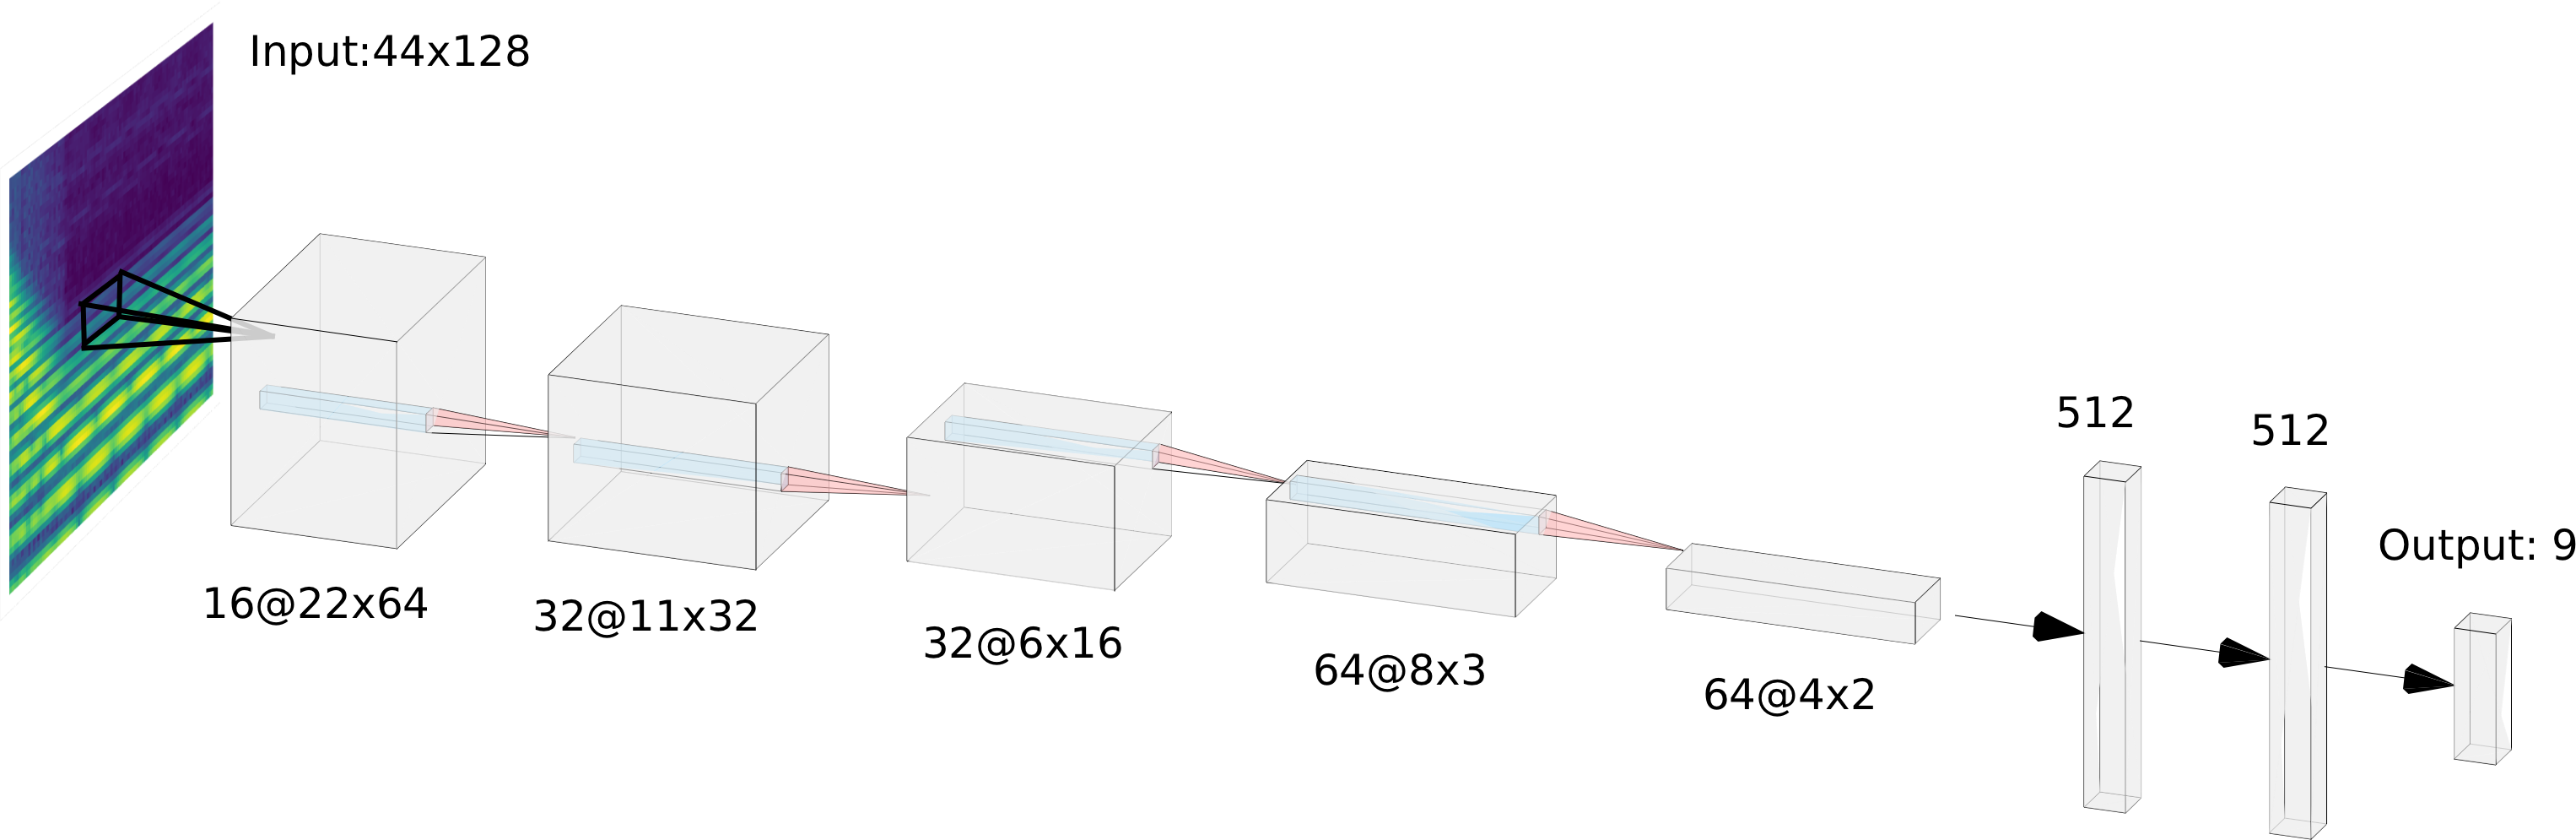
\includegraphics[width=0.99\textwidth]{figures/inverse-synth/CONV5s_Diagram.png}
    \caption{Network diagram of the Conv5s CNN. This model accepts a Mel-spectrogram as input and contains five 2D convolutional layers followed by two dense layers. The output layer is predicted synthesizer parameters.}
    \label{fig:conv5s}
\end{figure}

During initial experiments all of the models (especially the models with more capacity) began to overfit during training after about 50 epochs. A learning rate schedule was introduced in an attempt to address this and allow the models to train for longer. An inverse time-decay scheduler was included that reduced the learning rate according to the following equation:

\begin{align}
    \eta_i = \frac{\eta_0}{1 + \lambda\frac{i}{T}}
\end{align}

Where $\eta_i$ is the learning rate at training step $i$, $\eta_0$ is the initial learning rate, $\lambda$ is the decay rate, and $T$ is the decay steps. For this experiment $\eta_0=0.001$, $\lambda=1.0$, and $T$ was set to be equivalent to 50 epochs, which means that the decay rate decreased by a factor of two by 50 epochs into training. All the CNNs were trained using this learning schedule, an early-stopping patience of 20, and a batch-size of 128. 

% Three models derived from work by Yee-King et al. \cite{yee2018automatic} were used: 1) A simple multi-layer perceptron with three hidden layers, all with a ReLu activation, 2) a LSTM recurrent network with three layers and dense output, and 3) a LSTM++ networks which contains a single bidirectional LSTM node followed by a dense layer with an elu activation, six highway layers, and a dense output. One convolutional neural network (CNN) derived from work by Barkan et al. \cite{barkan2019inversynth} was also included: this network featured six layers of strided convolutions followed by a dropout layer and a dense output. Specific details of all these models is provided in appendx \ref{appendix:spiegelib_models}.

% Models were trained using an $Adam$ optimizer \cite{kingma2014adam} with a learning rate of 0.001, batch sizes of 64, and used an early stopping callback which halted training if validation loss was stagnant for 10 epochs to prevent overfitting. Ideally the loss function would be computed directly on audio rendered from $Dexed$ using the predicted parameters, but that is challenging to implement, so the loss is computed on the parameter values which has been standard in previous work \cite{yee2018automatic, barkan2019inversynth}.

% The loss function used was the RMS error between the target parameter values and the predicted parameter values, which is given by the following formula where $N$ is the number parameters, $\textbf{y}$ is the true parameter values, and $\hat{\textbf{y}}$ is the predicted parameter values:



% Logging of training and validation progress was recorded using the \mintinline{python}{TFEpochLogger} class. Plots of training and validation accuracy and loss for the LSTM++ model are shown in figure \ref{fig:lstm_bi_train}. 

% % TODO: add in some of the other loss plots (probably all of them) and remark on the differences betwee them.

% Trained models are then saved for future use.

% \begin{figure}[ht]
% \begin{center}
% 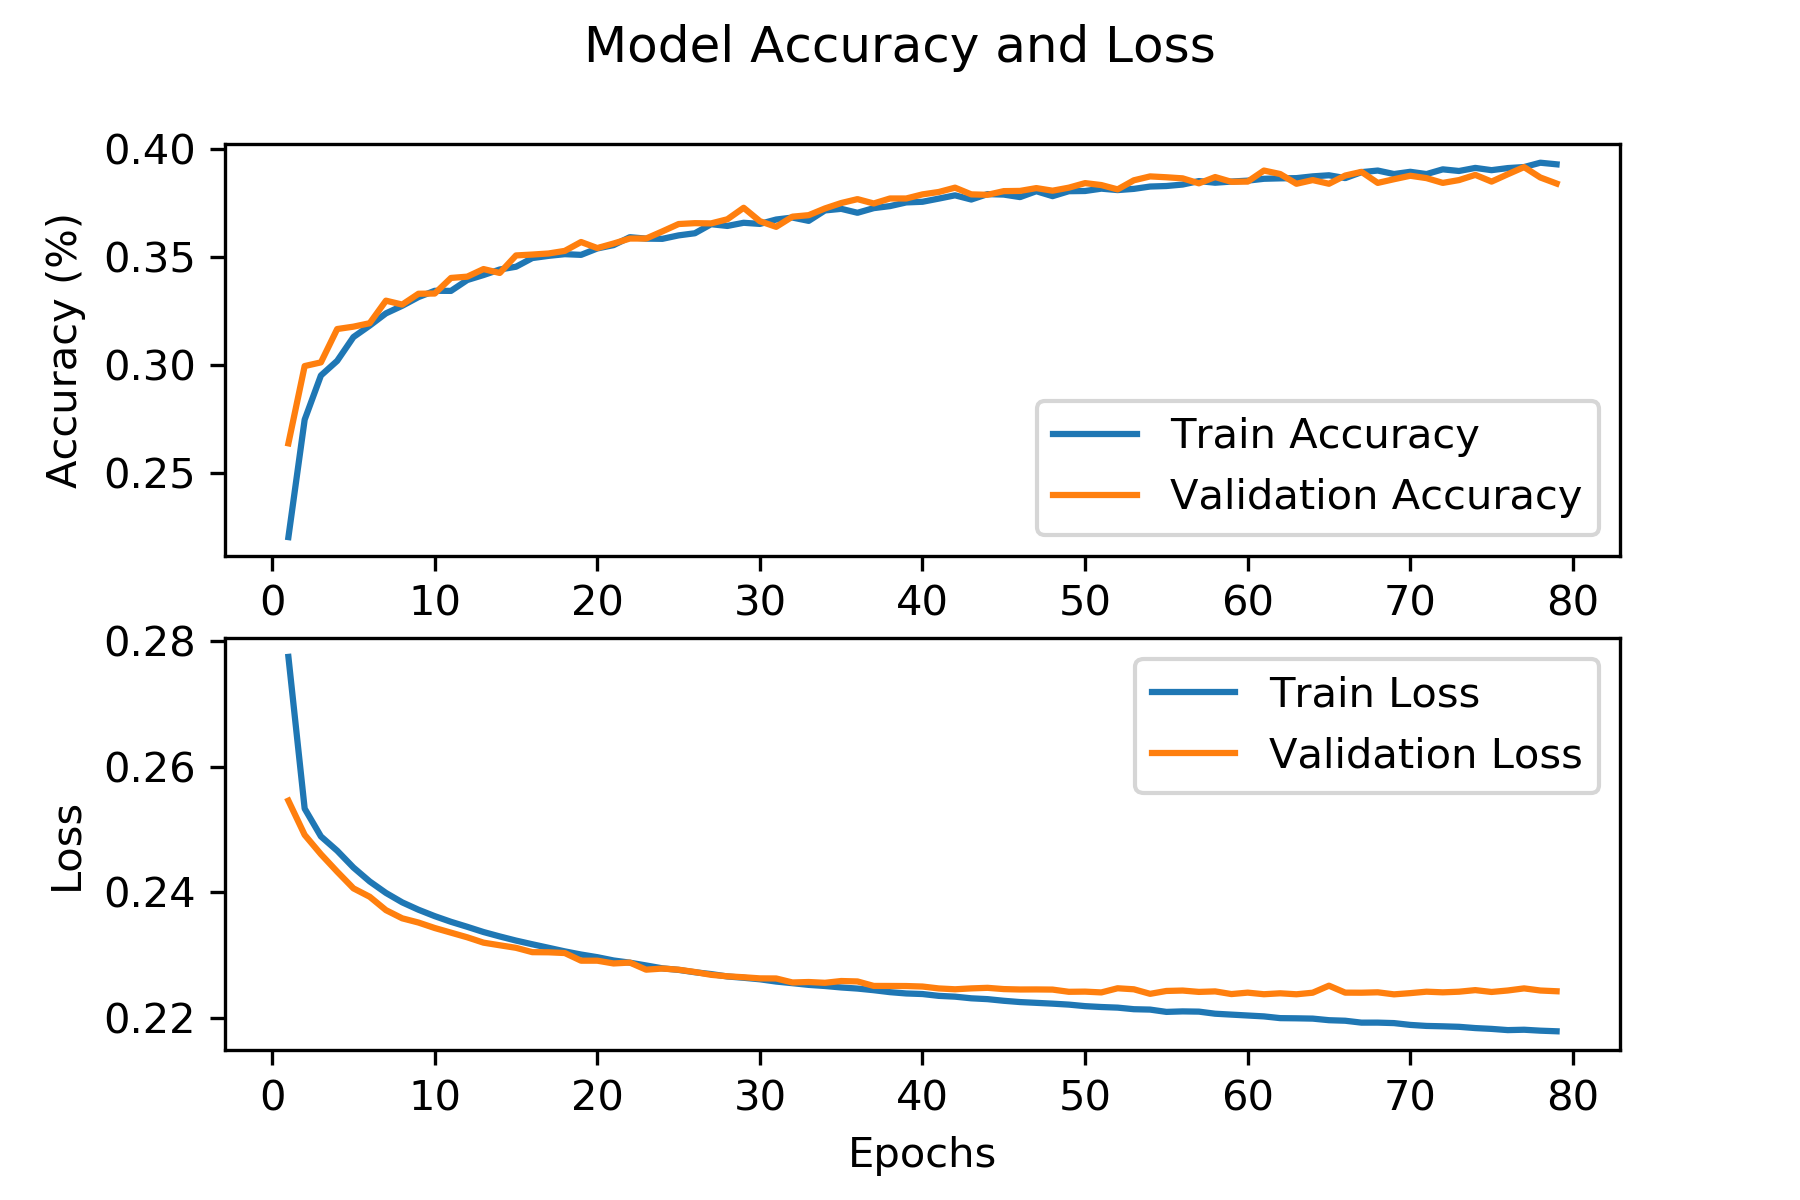
\includegraphics[width=0.75\columnwidth]{blstm_training.png}
% \caption{Traing and validation accuracy and loss over epochs for LSTM++ model training.}
% \label{fig:lstm_bi_train}
% \end{center}
% \end{figure}

\subsection{Genetic Algorithms}
Two different GAs were used: a basic single-objective GA and a multi-objective NSGA III. The multi-ojective GA was derived from work conducted by \cite{macret2012automatic} that used the algorithm to automatically tune the parameters of a Teenage Engineering OP-1\footnote{\url{https://teenage.engineering/products/op-1}} synthesizer. In the GAs the $fitness$ is easily computed directly on the audio rendered from $Dexed$.

In the case of the basic GA the $fitness$ is computed as the mean absolute error (MAE) between 13-band MFCCs from the target and the individual. Three different metrics were used for evaluating the $fitness$ of an individual for the NSGA-III algorithm, MAE between: 1) a 13-band MFCC, 2) magnitude spectrum from an FFT, and 3) five spectral features. MAE is given by the following formula, where $N$ is the number of features, $y$ is the target, and $\hat{y}$ is the predicted individual:

\begin{equation}
    \text{MAE} = \frac{\sum_{i \in N}{|y_i - \hat{y}_i|}}{N}
\end{equation}

Both genetic algorithms were run for 100 generations for each sound target. The basic GA and NSGA used population sizes of 300 and 100 individuals respectively. 

%Figure \ref{fig:nsga_fitness} shows the minimum spectral error achieved by an individual during each iteration of the NSGA algorithm on one of the target sounds. The plot shows a period of rapid improvement during early iterations, with some short periods of stagnation, followed by longer periods where the algorithm is unable to find an individual that is an improvement over those in the current population.

% TODO: Add in the other population generation plots for each objective

\begin{figure}[ht]
\begin{center}
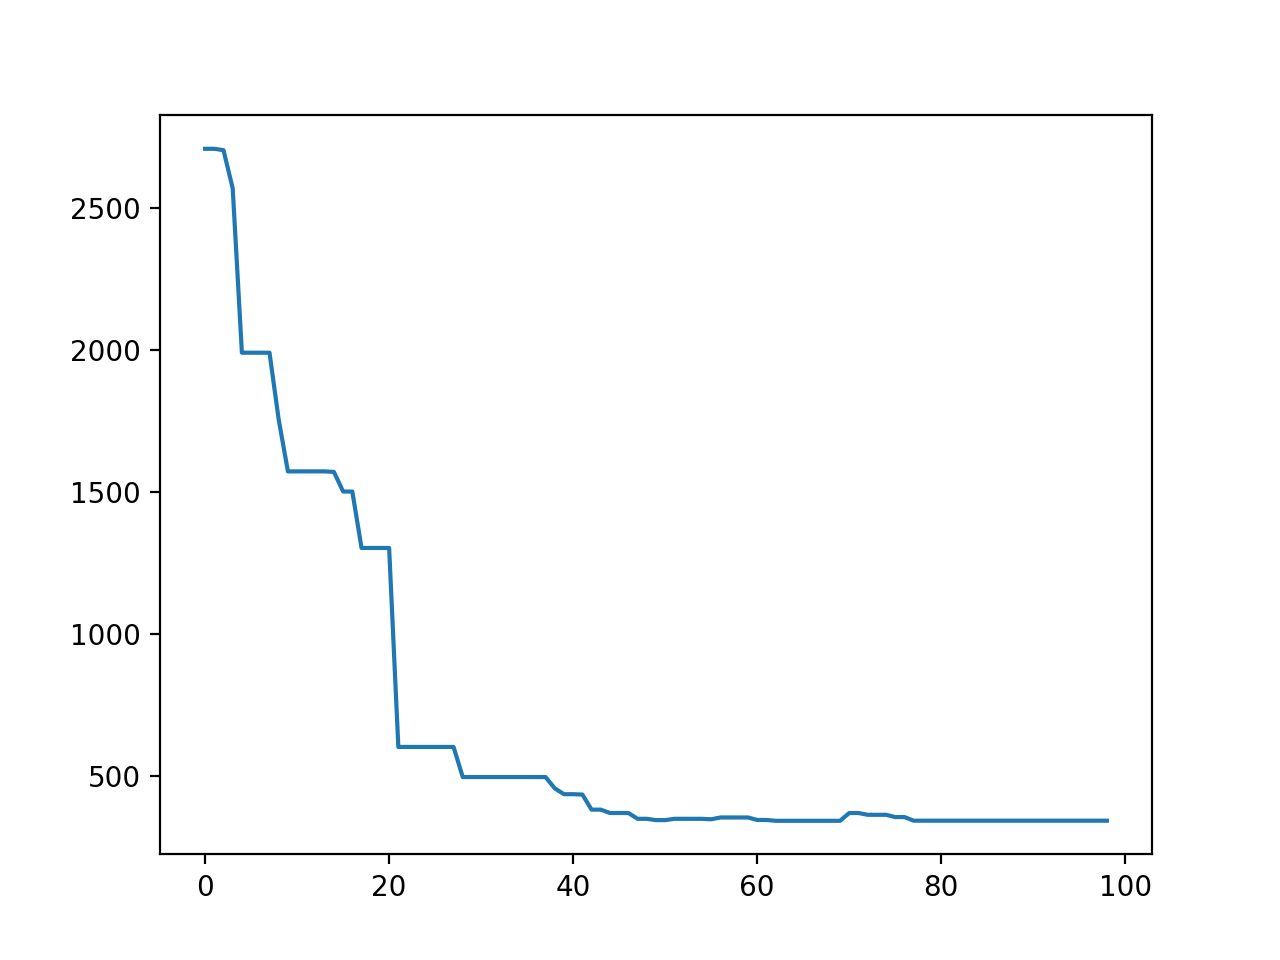
\includegraphics[width=0.7\columnwidth]{nsga_target_15_FFT.png}
\caption{Minimum FFT MAE in the population at each generation to target sound 15 for NSGA III estimator.}
\label{fig:nsga_fitness}
\end{center}
\end{figure}

\section{Evaluation}
\label{sec:inverse-synth-eval}

To evaluate each of the techniques an evaluation dataset containing 25 random sounds generated using the same nine-parameter $Dexed$ configuration was used. Using the sounds generated using the same synthesizer configuration means that an error of zero is possible, which provides a stable baseline for comparing each of the methods. All estimators were run on each one of the 25 target sounds using the \mintinline{python}{SoundMatch} class. This resulted in a set of audio files generated from $Dexed$ using the estimated parameters from each estimator run on each of the 25 target sounds. All of the resulting sounds are available for listening online on the SpiegeLib docs page\footnote{\url{https://spiegelib.github.io/spiegelib/examples/fm_sound_match_pages/fm_sound_match_listen.html}}. Quantitative and qualitative evaluation was conducted on these sounds.

\subsection{Quantitative Evaluation}
Evaluation was conducted by comparing the predicted audio files to the target audio using MAE computed on MFCCs, which is the same method that was used during evaluation by Yee-King et al. \cite{yee2018automatic}. Results for mean absolute error (MAE) which have been summarized using mean, standard deviation, minimum, and maximum, are shown for each estimator in table \ref{tbl:sound_match_eval}. Both GAs performed better than the deep learning approaches with the NSGA III having the best overall score. For deep learning approaches, the LSTM++ model achieved the best mean score.

\begin{table}[t]
\centering
\caption{Results from sound matching evaluation}
\label{tbl:sound_match_eval}
\begin{threeparttable}
\begin{tabular}{l|cccc}
\toprule
$Method$ & $Mean$ & $SD$ & $Min$ & $Max$ \\
\midrule
$MLP$ & 8.55 & 6.77 & 1.92 & 34.12 \\
$CNN$ & 7.88 & 4.26 & 2.68 & 20.89 \\
$LSTM$ & 6.12 & 3.76 & 1.20 & 19.36 \\
$LSTM++$ & 4.91 & 6.50 & 2.12 & 21.51 \\
$GA$ & 2.25 & 2.58 & 0.70 & 11.17 \\
$NSGA III$ & \textbf{0.81} & \textbf{0.89} & \textbf{0.001} & \textbf{3.06} \\
\bottomrule
\end{tabular}
\begin{tablenotes}[para, flushleft]
\footnotesize
\item Values shown are calculated from the mean absolute error (MAE) calculated during MFCC evaluation. Smaller MAE values indicate more similar matches. The NSGA III estimator received the best scores, which are shown in bold font.
\end{tablenotes}
\end{threeparttable}
%\vspace{5mm}
\end{table}

% TODO informal listening based on MAE so I can comment on the results in terms of MAE

Histograms of the the MAE were also plotted for each estimator using the \mintinline{python}{plot_hist()} method in \mintinline{python}{EvaluationBase}. Histograms of the MAE for all predictions made by all estimators are shown in figure \ref{fig:group_hist}. These plots clearly show the NSGA III as the winner in terms of MFCC MAE; 24/25 of the predicted sounds have an MAE less than 2.5 (the smallest histogram bin), and the other sound is still less than 5. For the deep learning models, the LSTM++ performed the best overall, however the LSTM model produced more results that had a MAE less than 2.5. The MLP model performed the worst overall and the histogram shows a wide range of results, the MLP also produced a result with the worst individual score of 34.12. The CNN model performed only slightly better than the MLP and had no predictions with a score less than 2.5.

\begin{table}[t]
\centering
\caption{Results from sound matching evaluation}
\label{tbl:param_eval_eg}
\begin{tabular}{r|ccc|ccc|c}
\toprule
{} & \multicolumn{3}{c}{EG RATE} & \multicolumn{3}{c}{EG LEVEL} & {} \\
{} & 2 & 3 & 4 & 2 & 3 & 4 & Mean \\
\midrule
MLP      &     0.0011 &     0.0902 &     0.0223 &      0.0096 &      0.0134 &      0.0215 &   0.0264 \\
LSTM     &     0.0002 &     \textbf{0.0081} &     0.0191 &      0.0042 &      0.0020 &      0.0331 &   0.0111 \\
5-LSTM++ &     0.0007 &     0.0354 &     0.0210 &      0.0069 &      0.0037 &      0.0348 &   0.0171 \\
LSTM++   &     \textbf{0.0002} &     0.0241 &     0.0306 &      0.0072 &      0.0025 &      0.0434 &   0.0180 \\
Conv6    &     0.0022 &     0.0212 &     0.0583 &      0.0024 &      0.0071 &      0.0223 &   0.0189 \\
Conv6s   &     0.0008 &     0.0252 &     0.0280 &      0.0107 &      0.0029 &      0.0307 &   0.0164 \\
Conv5    &     0.0026 &     0.0230 &     0.0300 &      0.0055 &      0.0108 &      0.0321 &   0.0174 \\
Conv5s   &     0.0012 &     0.0293 &     0.0111 &      0.0067 &      0.0033 &      0.0228 &   0.0124 \\
\midrule
Mean  &     0.0011 &     0.0321 &     0.0275 &      0.0067 &      0.0057 &      0.0301 &   0.0172 \\
\bottomrule
\end{tabular}
\end{table}

\begin{table}[t]
\centering
\caption{Results from sound matching evaluation}
\label{tbl:param_eval_osc}
\begin{tabular}{r|ccc|c}
\toprule
{} & \multicolumn{3}{c}{OSC} & {} \\
{} & Coarse & Fine & Detune & Mean \\
\midrule
MLP      &    0.0053 &  0.0958 &      0.0709 & 0.0573 \\
LSTM     &    0.0044 &  0.0770 &      0.0606 & 0.0473 \\
5-LSTM++ &    0.0056 &  0.0696 &      0.0711 & 0.0488 \\
LSTM++   &    0.0052 &  0.0933 &      0.0723 & 0.0570 \\
Conv6    &    0.0051 &  0.0852 &      0.0681 & 0.0528 \\
Conv6s   &    0.0063 &  0.0916 &      0.0651 & 0.0543 \\
Conv5    &    0.0093 &  0.0698 &      0.0721 & 0.0504 \\
Conv5s   &    0.0068 &  0.0729 &      0.0704 & 0.0500 \\
\midrule
Mean     &    0.0060 &  0.0819 &      0.0689 & 0.0523 \\
\bottomrule
\end{tabular}
\end{table}
% TODO objective evaluation based on the parameter values?

\subsection{Qualitative Evaluation}
Spectrograms of one target sound and predictions made by each of the estimators for that target are shown in figure \ref{fig:group_spect}. The selected example was one of the most challenging targets; both the GAs, the LSTM, and the MLP received their worst individual score on it. The most clear difference between the spectrograms can be seen in the temporal evaluation of the harmonics, which is caused by the EG applied to the amplitude of the second operator. In the target the envelope has two obvious components: 1) gradually descending over the first half, and then 2) remaining constant for the remainder of the sound. All the predictions have a similar shape, however only the NSGA III is able to match the shape of of those two sections of the envelope. The MLP, which performed the worst, has two envelope sections, but the first section descends too radpidly and then the constant section is at the incorrect amplitude.

Another aspect of the spectrograms that can be identified are periodic amplitude modulations occuring along the horizontal axis of the harmonics. These show up as period dark notches on the harmonic. These spacing between the horizontal notches indicates the tuning of the second operator that is modulating the frequency of the first operator. In the target this modulation pattern shows up in the first half of the clip, but not the second. Only the NSGA III was able to correctly match the tuning in both sections of the audio. 

% Did I mess up the charts for the CNN and the GA?? Those shouldn't be different I don't think?

\begin{figure}[t]
\begin{center}
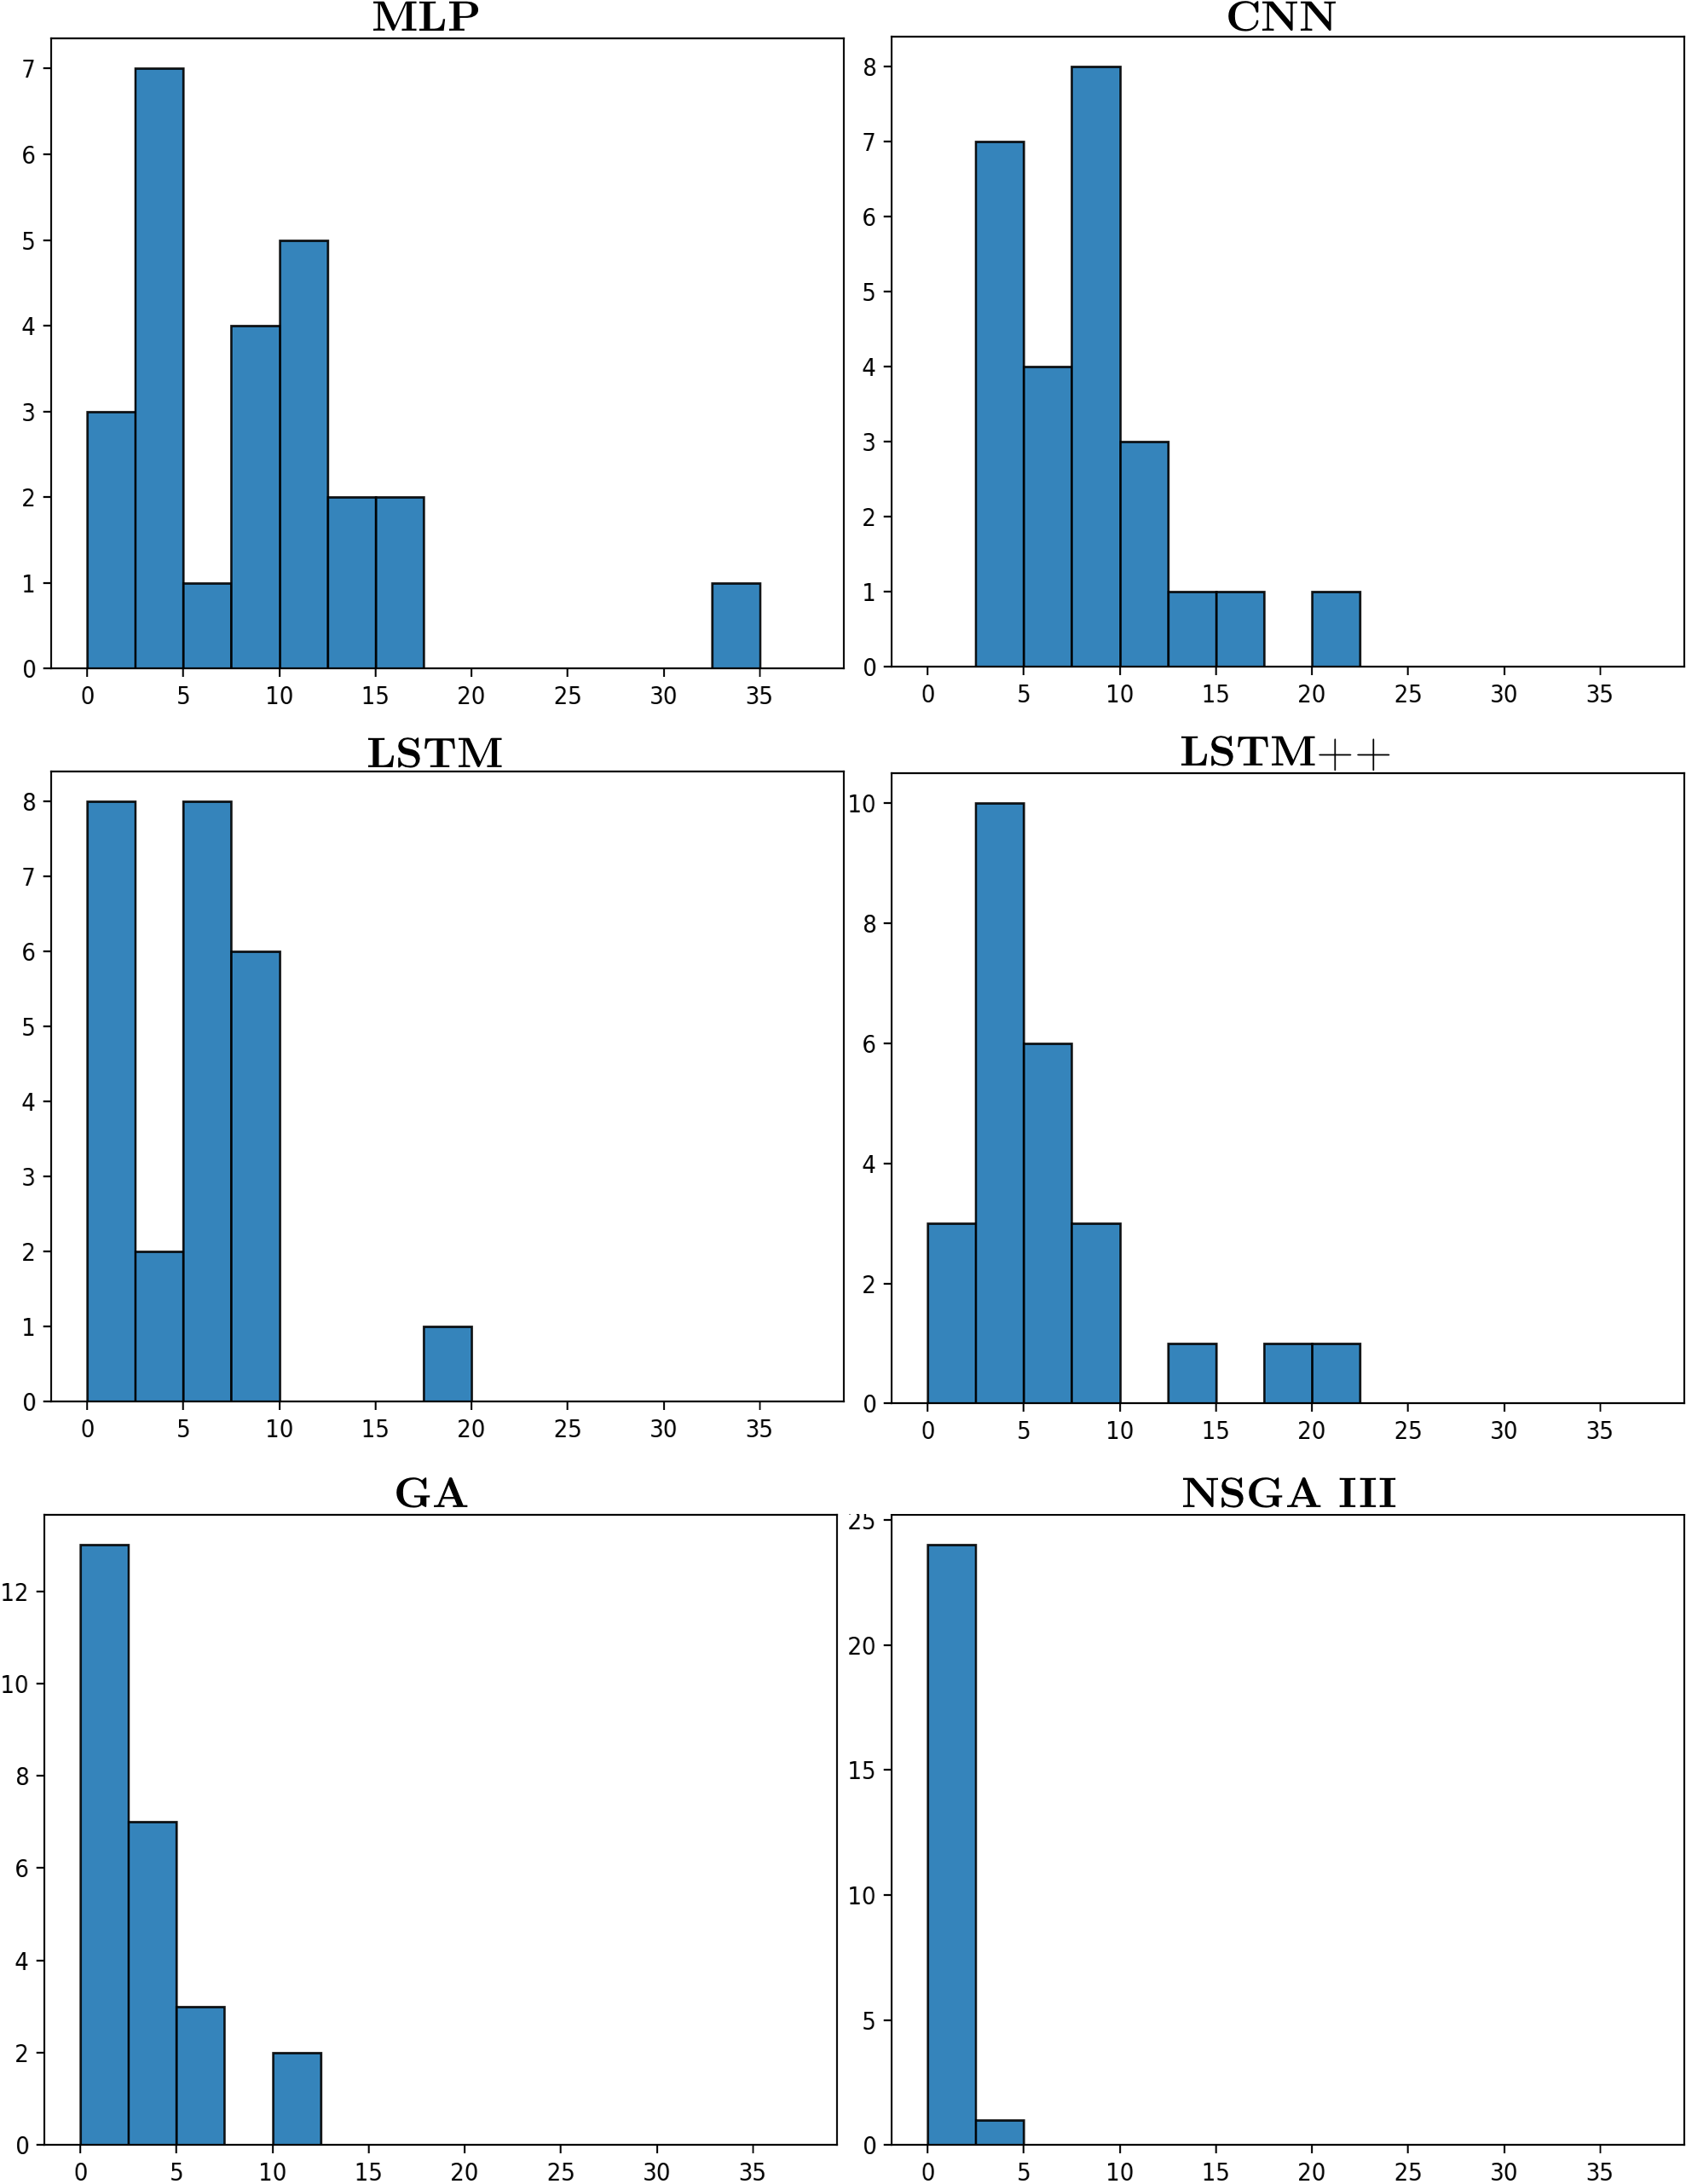
\includegraphics[width=0.75\textwidth]{hist_group_v3.png}
\caption{Histogram shows the MAE values resulting from MFCC evaluation run on a set of 25 sound targets for all estimators. Lower MAE values indicate a closer sound match.}
\label{fig:group_hist}
\end{center}
\end{figure}

\begin{figure}[t]
\begin{center}
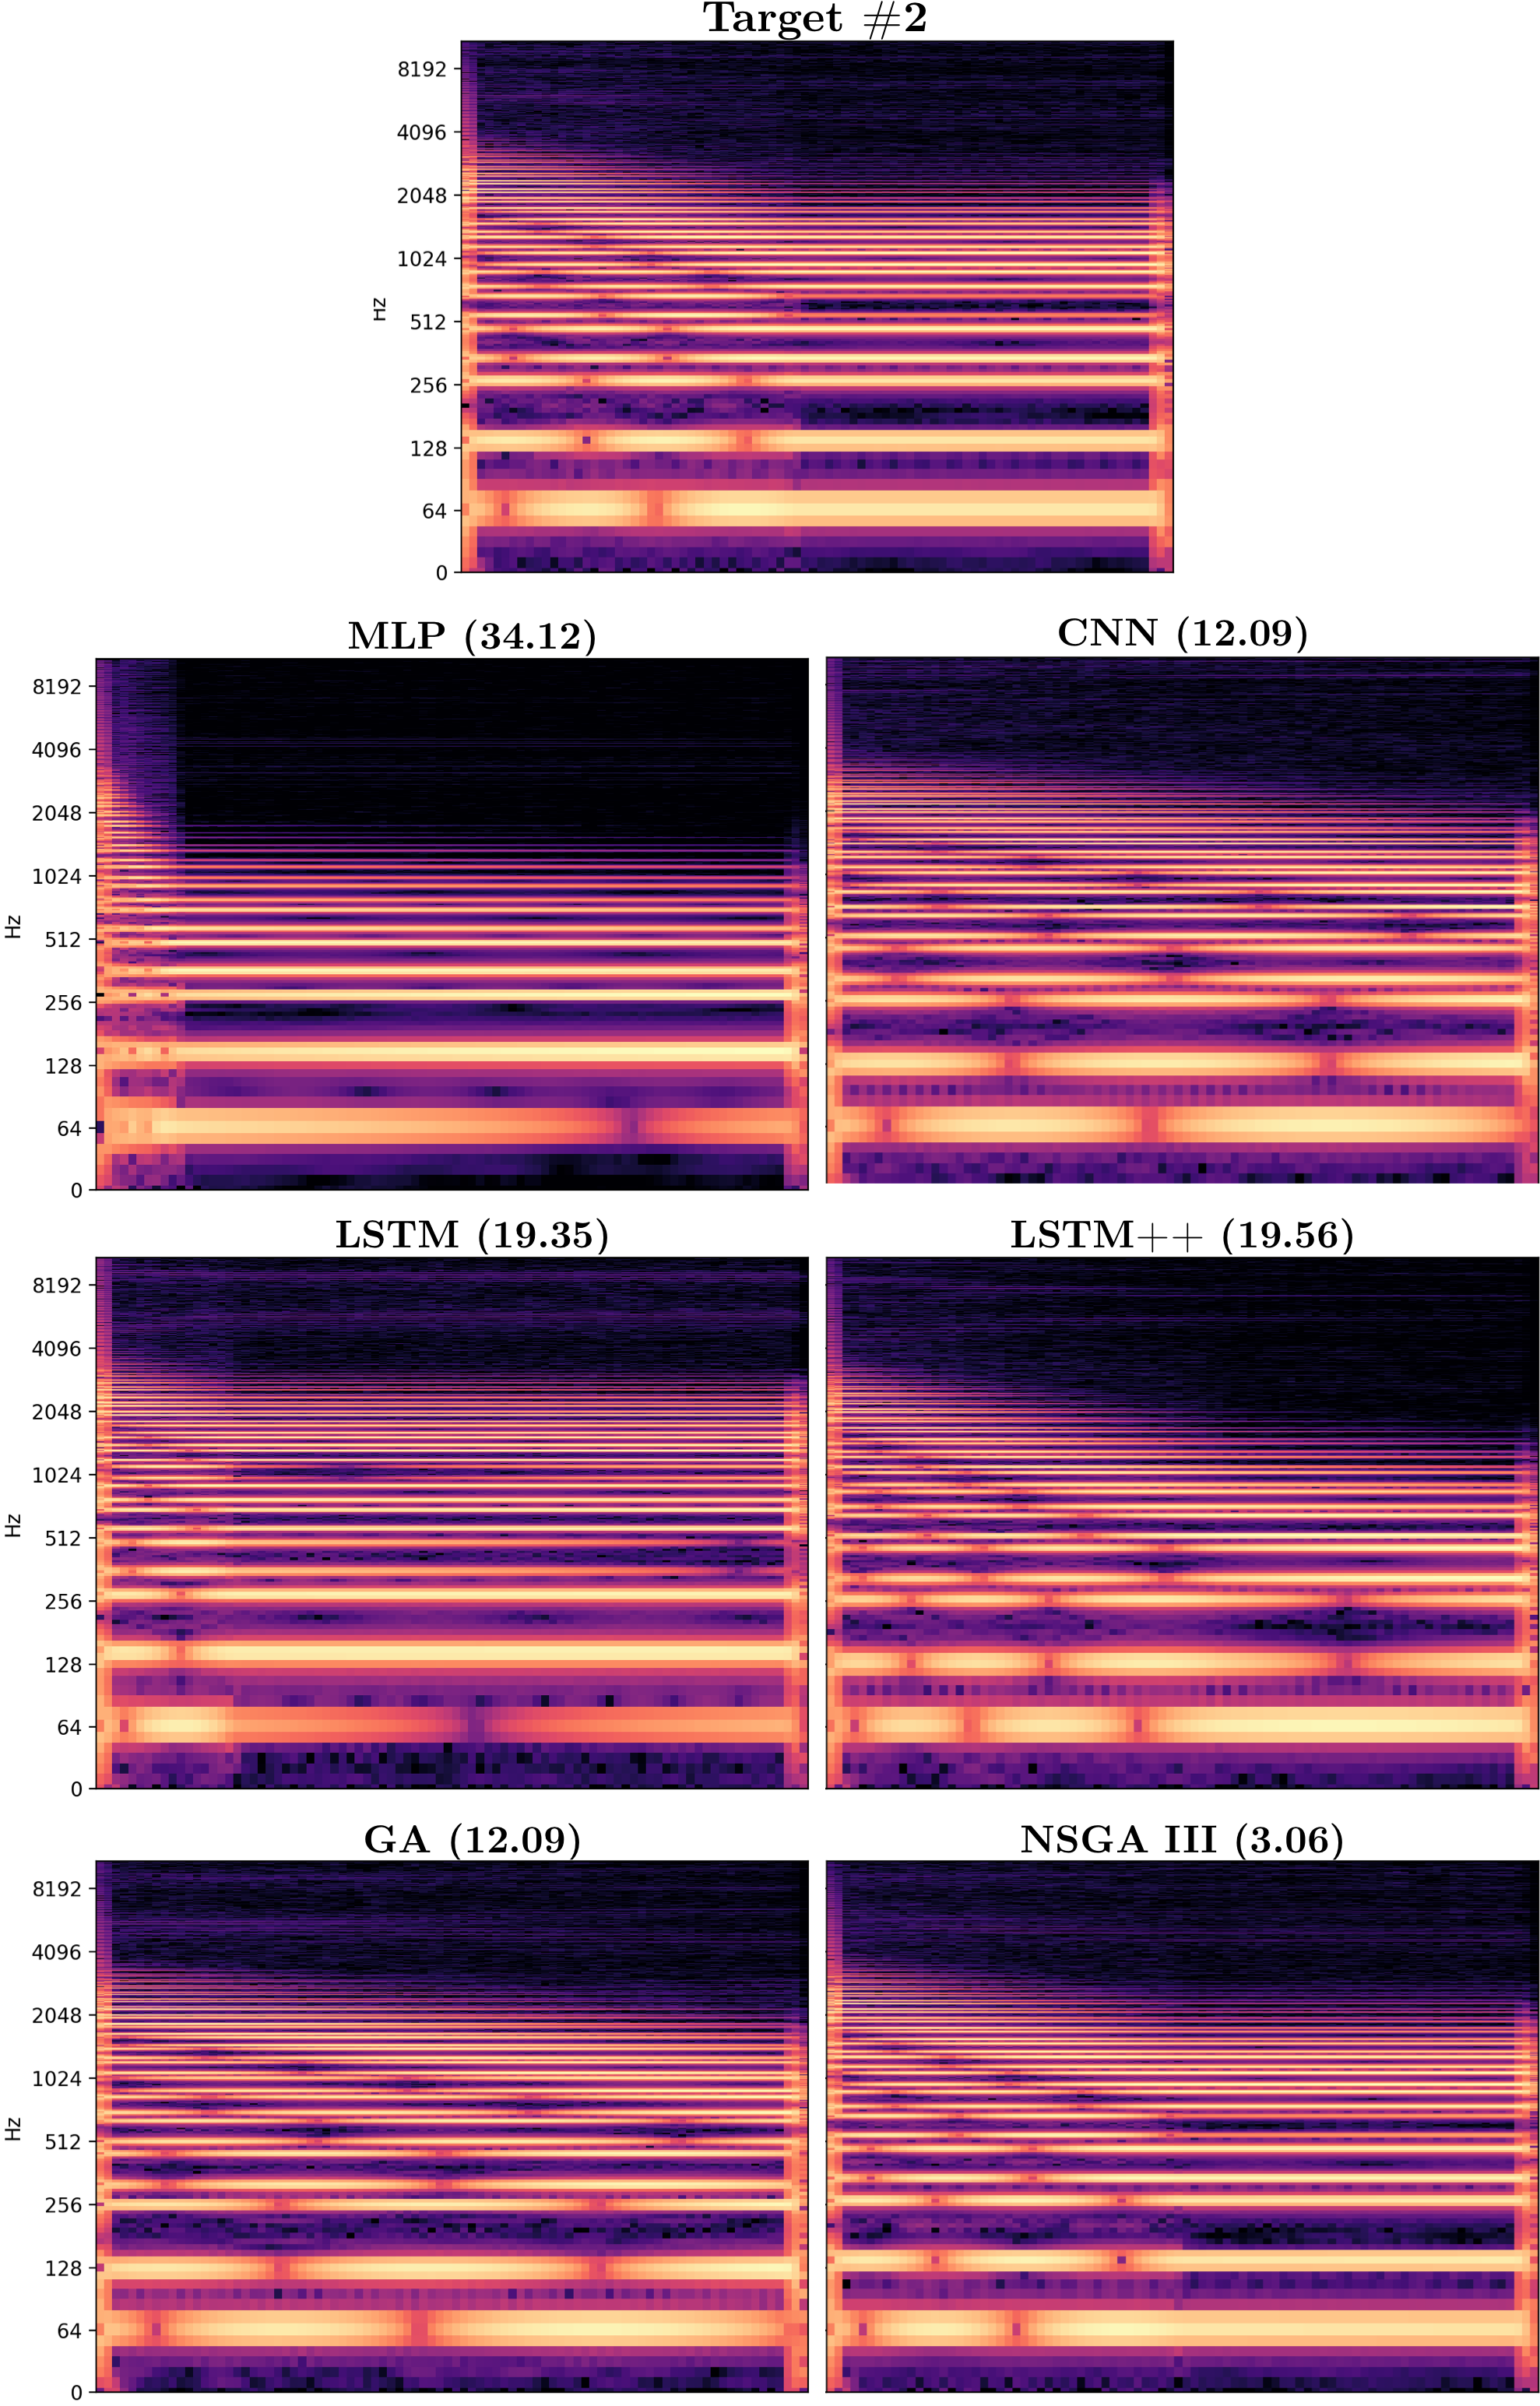
\includegraphics[width=0.75\textwidth]{spect_group_v1.png}
\caption{Spectrogram plots of a target sound and sound match predictions made by each estimator. The value next to the estimator name is the MAE value from MFCC evaluation for that prediction (lower MAE values indicate a closer match).}
\label{fig:group_spect}
\end{center}
\end{figure}

% I think this can be removed?
% To evaluate to the resulting predictions the \mintinline{python}{MFCCEval} class was used, which calculates error and distance metrics on MFCCs of a target and prediction. Results for mean absolute error (MAE) which have been summarized using mean, standard deviation, minimum, and maximum, are shown for each estimator in table \ref{tbl:sound_match_eval}. Both GAs performed better than the deep learning approaches with the NSGA III having the best overall score. For deep learning approaches, the LSTM++ model achieved the best mean score. Histograms of the the MAE were also plotted for each estimator using the \mintinline{python}{plot_hist()} method in \mintinline{python}{EvaluationBase}. Histograms of the MAE for all predictions made by all estimators are shown in figure \ref{fig:group_hist}. Spectrograms of one target sound and sound match predictions made by each of the estimators for that target are shown in figure \ref{fig:group_spect}. For this particular target, spectrograms reveal that while the frequency and distribution of the harmonics was relatively close for each estimation, all estimators except for the NSGA III struggled with matching the temporal envelope of the spectrum.

\section{Discussion}
\label{sec:inverse-synth-discuss}


\section{Conclusion}

- Conducted an inverse synthesis experiment on a VST software synthesizer Dexed
- Results showed that the GAs performed the best via objective evaluation
- LSTM++ model performed the best out of the deep learning models
- Comparison of the search versus modelling methods for inverse synthesis
- Discussion of the parameter sampling methods -- uniform sampling may not provide the best method for training the deep learning models to learn sounds that a human might program
- Challenges associated with programming a VST software synth




%\section{Related Work}
%- Go over the three specific papers that SpiegeLib and the experiments are based on.
%- Deep learning: Fully connected and recursive nets: \cite{yee2018automatic}, Convolutional Nets: \cite{barkan2019inversynth}, Genetic Algorithms: \cite{tatar2016automatic}
%
%\subsection{Recurrent Neural Networks}
%One of the first works on the application of deep learning to the inverse synthesis problem was published by Matthew Yee-King et al. \cite{yee2018automatic} in 2018. The main contribution of their work was an experiment that showed the effectiveness of a type of recurrent neural networks (RNN) called long short-term memory (LSTM) networks at sound matching on an FM synthesizer audio plugin. RNNs were developed to handle time-series data and receive ordered data which is successively fed into the network architecture. As data is fed into the networks, activation states are stored internally and help to provide temporal context in latter stages of computation. RNNs have been particularly successful for audio generation problems \cite{oord2016wavenet, engel2017neural}. 
%
%Yee-King er al. also experimented with additional machine learning techniques including genetic algorithm (GA), Hill-climber, and  multi-layer perceptron (MLP) methods. They also compared two RNN models: a regular LSTM network as well as a modified LSTM network that had a bi-directional LSTM layer as well as several highway layers, they called this network an LSTM++. Their methodology compared a set of algorithms on a series of successfully more challenging problems on the open-source FM synthesizer Dexed\footnote{\url{https://asb2m10.github.io/dexed/}}. Each problem was focused on programming a subset of the parameters in Dexed; a larger subset was used for each successive problem. A dataset of audio samples paired with the parameters used to generate the audio was created for training each of the deep learning models. Mel-frequency Cepstral Coefficients (MFCCs) were used as input for each of the models. The results were evaluated by looking at the error between MFCCs from target sound and a predicted sound. Results showed that the hill-climber algorithm and the LSTM++ model performed the best. The LSTM++ model showed significant improvements over the other deep learning methods, however the hill-climber performed the best on a majority of the tasks.
%
%Their methodology and software provided a basis for the work presented in the chapter and in the development of SpiegeLib.
%
%\subsection{Convolutional Neural Networks}
%Barkan et al. explored convolutional neural networks (CNNs) applied to the inverse synthesis problem in their work which presenting InverSynth \cite{barkan2019deep}. The CNN has been used extensively for image related deep learning tasks and has recently been used successfully in music and audio related tasks including music genre classification \cite{choi2016automatic} and neural audio generation \cite{donahue2018adversarial}. A key feature of CNNs is the use of shared filters that perform convolutions and produce representations at various levels of specificity. The shared filters has allowed them to process large input data such as images and audio with relatively few parameters compared to their fully connected counterparts. 
%
%In their work, Barkan et al. experiment with several different CNN architectures and compare them to a few different fully-connected networks. The focus of their research is performing inverse synthesis on a custom built four oscillator FM synthesizer. They frame the inverse synthesis problem as a classification problem and quantize each of the 23 continuous synthesizer parameters into 16 discrete states. As input they experiment with both STFT as well as raw time-domain audio. Because of the size of these input they created different input representations for the fully-connected networks, for these they used a selection of hand-picked audio features defined in work by Itoyama et al. \cite{itoyama2014parameter}.
%
%Results were evaluated using four different objective methods which evaluate both the ability of the model to match the parameters as well as to reconstruct the target audio. The evaluation metrics used are:
%1) Mean Percentile Rank (MPR): ranked position of the correct class measured against predicted classes in the output. Computed independently on each of the 23 synthesizer parameters, each parameter has 16 classes.
%2) Top-k Mean Accuracy: measures whether the correct class is among the top-k predicted classes for each parameter.
%3) Mean Absolute Error (MAE): this measures the error of the predicted class for each parameter.
%4) Spectral Reconstruction Quality: predicted parameters are used to synthesize a predicted audio. The predicted audio is compared against the target audio using error metrics calculated on the STFT and FT representations.
%
%They also conducted a subjective listening experiment which measured the quality of the target audio to the predicted audio for a selection of the methods. Results from the objective and subjective evaluation showed that the depth of the convolutional network played an important role in the quality of the estimator and the best performing networks were two different networks with 6-layers.